\documentclass[../EDF Master Thesis.tex]{subfiles}

\begin{document}

Die \ac{dft} kann ein zeitdiskretes Signal in dessen Frequenzteile (Spektrum) aufspalten, wie in \autoref{fig:aufspaltung_eines_Signals_in_dessen_Frequenzteile} dargestellt. Dies ist sehr nützlich für viele Bereiche der Signalverarbeitung \ac{zb} für das Komprimieren von Musikaufnahmen, wo nicht hörbare Frequenzen rausgefiltert werden.

\begin{figure}[ht!]
    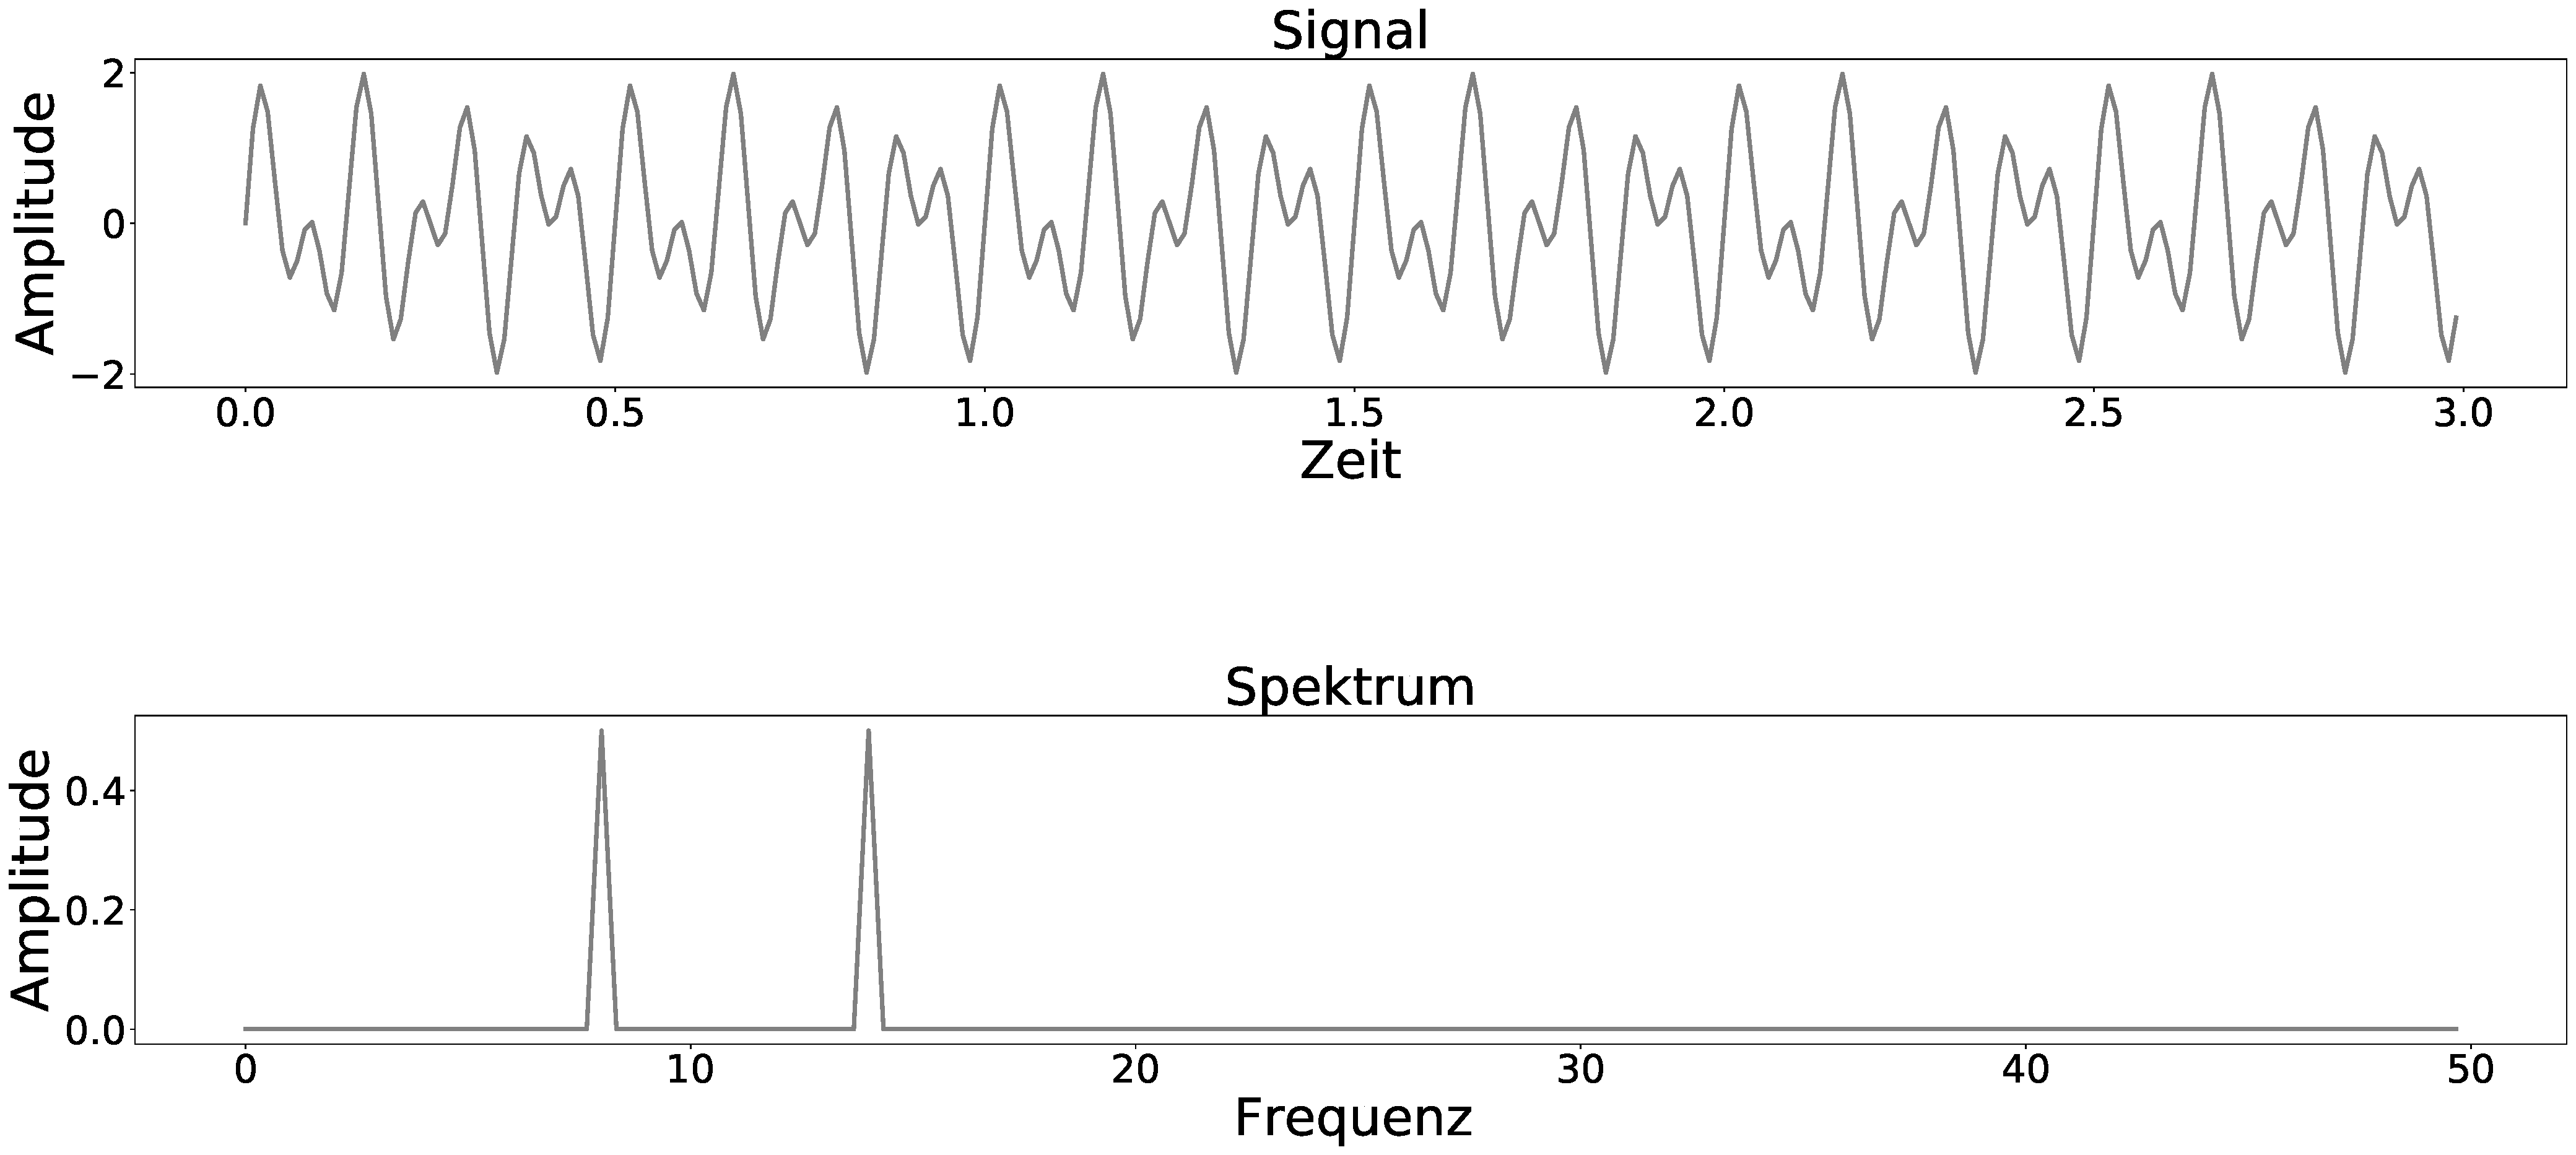
\includegraphics[width=1\textwidth]{attachments/fft_example.pdf}
    \caption{Aufspaltung eines Signals in dessen Frequenzteile}
    \label{fig:aufspaltung_eines_Signals_in_dessen_Frequenzteile}
\end{figure}

Bei der Berechnung einer \ac{dft} steigt dessen Komplexität $O$ mit der Anzahl der Abtastpunkte $N$ quadratisch an, wie in der \autoref{form:berechnung_der_dft_komplexitaet} dargestellt.
Dies führt dazu, dass eine reine Berechnung mit Hilfe der \ac{dft} auf kleinen Mikrocontrollern häufig nicht praktikabel ist.

\begin{equ}[ht!]
    \begin{equation}
        O(N) = (N^2)
    \end{equation}
    \caption{Berechnung der \ac{dft} Komplexität}
    \label{form:berechnung_der_dft_komplexitaet}
\end{equ}


Im Gegensatz zur \ac{dft} stellt die \ac{fft} ein Algorithmus dar, mit der der Rechenaufwand deutlich reduziert wird.
Aus diesem Grund wird häufig die \ac{fft} benutzt, die nach dem 'Teile und Herrsche'-Verfahren funktioniert und nur noch eine Komplexität von $O(N) = (N * log(N))$ besitzt \autocite{fft:001}.
Durch diese enorme Zeit- und Rechenersparnis fand die \ac{fft} in vielen Bereichen, wie \ac{zb} in Ingenieurswissenschaften, Musik, Wissenschaft und der Mathematik Verwendung \autocite{wiki:010}.
Für die Berechnung der \ac{fft} sind mehrere Algorithmen verfügbar, wobei in dieser Masterarbeit der Radix-2 Algorithmus von der \ac{cmsis}-\ac{dsp} Bibliothek verwendet wurde.
Als Vorraussetzung des Algorithmus der \ac{fft} muss die Anzahl der Messwerte $N$, auch Samples genannt, einer Zweierpotenz entsprechen.

\begin{equ}[ht!]
    \begin{equation}
        N = 2^N, N \in \mathbb{N}
    \end{equation}
    \begin{center}
        \begin{tabular}{lcr}
            $N$ & Anzahl von Samples \\
            $\in$ & natürliche Zahlen\\
        \end{tabular}
    \end{center}
    \caption{Rechenbedingung der \ac{fft}}
    \label{form:rechenbedingung_der_fft}
\end{equ}

Wird die Rechenbedingung in \autoref{form:rechenbedingung_der_fft} erfüllt, kann diese in zwei Teilsummen zerlegt werden, je eine für gerade und ungerade Indizes.

\begin{equ}[ht!]
    \begin{equation}
        X(k) = \sum_{n=0}^{N-1} x(n) \cdot w_N^{n \cdot k} = \sum_{n=0,2,...}^{N-2} x(n) \cdot w_N^{n \cdot k} +  \sum_{n=1,3,...}^{N-1} x(n) \cdot w_N^{n \cdot k}
    \end{equation}
    \begin{center}
        \begin{tabular}{lcr}
            $w = e ^ {-j \cdot \frac{2 \cdot \pi}{N}}$ & komplexer Drehfaktor der \ac{dft} \\
        \end{tabular}
    \end{center}
    \caption{Aufteilung der \ac{dft} \ac{iaa} \autocite{fft:002}}
    \label{form:aufteilung_der_dft}
\end{equ}

Anschließen wird eine Substitution wie folgt angewandt:

\begin{table}[ht!]
    \begin{center}
        \begin{tabular}{lcr}
            $n = 2m$ & für $n$ gerade \\
            $n = 2m + 1$ & für $n$ ungerade \\
            $M = N / 2$ & als Abkürzung 
        \end{tabular}
    \end{center}
    \caption{Substitution der \ac{dft} \ac{iaa} \autocite{fft:002}}
    \label{form:substitution_der_dft}
\end{table}

Und berücksichtigt folgende Umformungen:

\begin{equ}[ht!]
    \begin{equation}
        w_N^{2m \cdot k} = w_M^{m \cdot k} \qquad \text{und}\qquad w_N^{(2m + 1) \cdot k} = w_N^k \cdot w_M^{m \cdot k}
    \end{equation}
    \caption{Umformung \ac{dft} \ac{iaa} \autocite{fft:002}}
    \label{form:umformung_dft}
\end{equ}

Resultieren zwei Gleichungen mit der halben Länge:

\begin{equ}[ht!]
    \begin{equation}
        X(k) = \sum_{m=0}^{M-1} x(2m) \cdot w_M^{m \cdot k} + \sum_{m=0}^{M-1} x(2m + 1) \cdot w_M^{m \cdot k}
    \end{equation}
    \caption{Resultierende Gleichungen nach Aufspaltung der \ac{dft} \ac{iaa} \autocite{fft:002}}
    \label{form:resultierende_gleichungen_nach_der_Aufspaltung_der_dft}
\end{equ}

Ist die resultierende Länge der \ac{dft} wieder eine Zweierpotenz, wird die Zerlegung solange fortgeführt, bis $N$ Vektoren der Länge $2^0$ erhält \autocite{fft:002}.
Anschließend werden die Ergebnisse zusammengerechnet und die \ac{dft} wurde gelöst.
\end{document}


